%---------------------导言区---------------------------%
\documentclass[12pt,a4paper,UTF8]{ctexart}
	%10pt:正文字体为12pt,缺省为10pt;各层级字体大小会根据正文字体自动调整
	%a4paper:纸张大小a4;
	%UTF8:中文要求
\usepackage{geometry}%用于设置上下左右页边距
	\geometry{left=2.5cm,right=2.5cm,top=3.2cm,bottom=2.8cm}
\usepackage{xeCJK,amsmath,paralist,enumerate,booktabs,multirow,graphicx,subfig,setspace,listings,lastpage,hyperref,amssymb,upgreek}
	%xeCJK:中文字体(如楷体,作者和机构需要用到)的设置
	%amsmath:数学公式
	%paralist,enumerate:自定义项目符号
	%booktabs:三线图,论文常用的表格风格
	%multirow:复杂表格
	%graphicx,float: 插入图片
	%subfig:并排排版图片、竖向排版图片
	%setspace:设置行间距等功能
	\setlength{\parindent}{2em}%正文首行缩进两个汉字
	%listings:用于排版各种代码;比如matlab的代码
	\lstset{language=Matlab}%matlab代码
	%lastpage:获取总页数;
	%hyperref:超链接,和lastpage搭配.
\usepackage{fancyhdr}
	%fancyhdr:一个很强大的宏包,用于自定义设计页面风格并命名以供调用。
	\pagestyle{fancy}
	\rhead{实验C2 原子定态能级的观测——弗兰克-赫兹实验}
	\lhead{基础物理实验\uppercase\expandafter{\romannumeral2}实验报告}
	\cfoot{Page \thepage/\pageref{LastPage}}  %当前页\总页数
		%分别是右页眉、左页眉、中页脚、右页脚
	\renewcommand{\headrulewidth}{0.4pt}
	\renewcommand{\theenumi}{(\arabic{enumi})}
	\setlength\headheight{15pt}

% \setCJKmainfont{FZShuSong-Z01S}[ItalicFont=FZKai-Z03S, BoldFont=FZHei-B01S]
%中文字体设置:使用开源字体方正书宋,方正楷体和方正黑体



%%%%%%%%%%%%%%%%%%%%%%%%%正文开始%%%%%%%%%%%%%%%%%%%%%%%%%%

\begin{document}

%%begin-------------------标题与信息-----------------------%%

%%标题
\begin{center}
\LARGE\textbf{实验C2 原子定态能级的观测—弗兰克-赫兹实验}
\end{center}

%%信息
\begin{doublespacing}
	%doublespacing:手动两倍行距
	\centering
	\begin{tabular}{lr}
	 & \\
	{\CJKfontspec{方正楷体简体} 学院:中山医学院} & {\CJKfontspec{方正楷体简体} 年级、专业:2020级临床医学(长学制)} \\
	{\CJKfontspec{方正楷体简体} 实验人姓名、学号:莫润冰~20980131} & {\CJKfontspec{方正楷体简体}合作者姓名、学号:黄健祥~20980118}\\
	{\CJKfontspec{方正楷体简体} 实验时间:2021年9月9日~星期四~上午} & {\CJKfontspec{方正楷体简体} 室温:28.8$^{\circ}$C~ 相对湿度:62\%}
	\end{tabular}
\end{doublespacing}

%%end-------------------标题与信息-----------------------%%


\subsection*{【实验目的】}
	%*表示不带上小节本身应有的1.1,下面的subsubsection*也是一样
%%自定义项目符号之(1)(2)(3)
	\begin{enumerate}[(1)]
		\item 学习弗兰克-赫兹(F-H)实验仪的使用方法
		\item 测量氩原子的电流-加速电压关系曲线,计算氩原子的第一激发电位
	\end{enumerate}

\subsection*{【仪器用具】}

%%一般表格
	%所有表格都可以通过Excel2LaTex加载项,在excel中转换成以下一串代码。需要琢磨的是调节一些细节的方法。

	% Table generated by Excel2LaTeX from sheet 'Sheet1'
	\begin{table}[htbp]
	  \centering
	    \begin{tabular}{cccp{20em}}
	    \toprule
	    编号    & 仪器用具名称 & 数量    & 主要参数(型号,测量范围,测量精度等) \\
	    \midrule
	    1     & 氩管 & 1     & ZKY-FH-Ar \\
		2     & 弗兰克-赫兹(F-H)实验仪  & 1     & ZKY-FH-4 \\
		3     &混合信号示波器 & 1 & RIGOLMSO2202A  \\
	    \bottomrule
	    \end{tabular}%
	  \label{tab:device}%
	\end{table}%

\subsection*{【实验原理】}

	\subsubsection*{1.F-H管内电子的碰撞过程}
%% 自然换段:\par,或者直接空一行,见107行和109行。
F-H实验的原理如图1(a)所示,其中充有汞蒸气的三极管称为弗兰克-赫兹管。
电子由热阴极管K发射,阴极K与栅极G之间的加速电压V$_{GK}$使电子加速,在阳极A与栅极G间加有反向推斥电压V$_{PG}$,管内空间的电位分布如图3所示。

当电子通过KG空间进入GA空间时,如果能量E$\geqslant$ eU$_{PG}$,就能冲过反向推斥电场到达阳极A,形成阳极电流,可由微电流计(pA)检出。
如果电子在KG空间与氩原子碰撞,把一部分能级传递给氩原子使其激发至高能级,则电子动能减小,在通过栅极后剩余的能量不足以克服反向推斥电场而被折回栅极,使通过微电流计的电流显著减小。
随着V$_{GK}$值继续增大,损失了部分动能的电子再次被加速,阳极电流增加,至电子与氩原子再次发生能量的交换。此过程多次反复,则阳极电流会出现周期性的变化在慢电子情况下,每一碰撞能交换的能量为氩原子的第一激发电位,记为U$_0$。
    % 两幅图并行排版,各有图题,还有一个总的图题
	% (1)注意正文中引用图片的方法,label可以打在minipage前面,也可以打在总图题的后面。
	% (2)需要调节图片大小,也可以调节位置。通过{minipage}后面的补充参数来调节位置。图片大小可以用高度来调以保证两个图高度一样。
	\begin{figure}[htbp]
		\centering
		\subfloat[实验电路图]{\label{fig:nogamma4}
		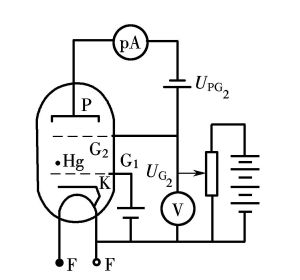
\includegraphics[width=0.4\textwidth]{img/1.jpg}%调节这里的图片宽度
		}%
		\subfloat[反射极电流与加速电压的关系]{\label{fig:withgamma4}
		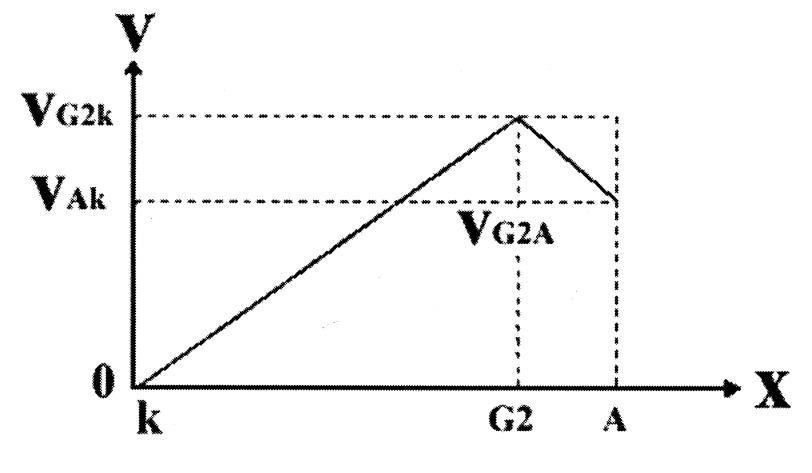
\includegraphics[width=0.4\textwidth]{img/2.jpg}%调节这里的图片宽度
		}%
		\caption{实验原理}
		\label{fig:tcvi}
	\end{figure}

	\subsubsection*{2.第一激发电位}
	
	图2所示的曲线为弗兰克-赫兹当年测得的电子在KG空间与汞原子进行能量传递的情况。
	该曲线有几个特征:

	\begin{figure}[htbp]
		\centering
		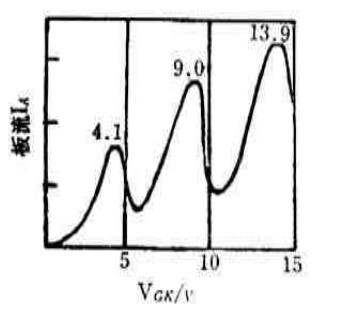
\includegraphics[width=0.4\textwidth]{img//3.jpg}
		\caption{管内空间电位分布}
	\end{figure}


%% paragraph后换段
	%paragraph后面的正文:无论是紧接着}敲还是换了几行,都会空一到两格后直接跟在后面。
	\paragraph{(1)}
	随V$_{GA}$的增加,反射级电流I$_A$显示出一系列极大值和极小值。
	\paragraph{(2)}
	各极大值(或极小值)之间的间距为4.9V,即汞原子的第一激发电位。对于别的原子,如单原子的惰性气体(He,Ne,Ar等)和单原子的金属蒸汽所做的实验,都能得到和图所示相似的结果。
	对仪器进行适当改进,还可以测出较高的激发电位和电离电位,进而证明原子内部能量状态的不连续性。
		% ~是一个控制符号,不会真的输出~,而是空一格。相应的,想要输出这个符号,就需要转义为\~。

	\subsubsection*{3.F-H发射光谱}	
	被慢电子激发碰撞到高能级的原子并不稳定,会跃迁回基态,并以光子的形式将激发态的能量eU$_{0}$向外辐射。
	对应光谱的波长为$eU_{0} = h\nu =\frac {hc}{\lambda }$ ,对于氩原子,$\lambda = \frac {hc}{eU_{0}}=108.1nm$ ,Ar的第一激发电位及谱线波长为11.6V,108.1nm。

	\subsubsection*{4.充氩F-H管最佳工作点的确定}
	在F-H实验中,影响I$_{A}$-V$_{G2K}$ 曲线的因素非常多。
	在采用外置式氩管进行实验时,无法改变工作物质的种类、管的结构和工作温度等,只能调节管个工作电压的数值。
	定性来说,灯丝电压决定发射总电子的多少, 起到手机热发射电子的作用;V$_{G2A}$将通过加速区而未到达阳极的电子推斥回栅极,起到抑制本地电流的作用,减小电离。
	曲线峰位和谷底的拟合曲线呈现纺锤的形状,若参数选择不合适,则 曲线的峰位拟合曲线尾部明显上翘,F-H管越容易电离。
	本实验将借助计算机和数据采集器,定量研究上述各种工作电压对 曲线的影响,在此定量研究的基础上,尝试找出一组最佳的工作参数,并与出场参数进行比较。
\subsection*{【实验内容及步骤】}

	\subsubsection*{1.基本操作}
	\begin{enumerate}[(1)]
			\item 开机并初始化机器,预热20-30min,“手动”指示灯亮。
			\item 选择电流量程,先取1$\upmu$A档,当“溢出”指示灯亮时再选更大量程。
			\item 设置氩管工作电压。
	\end{enumerate}

	\subsubsection*{2.氩元素第一激发电位的测量(手动测量)}
	\begin{enumerate}[(1)]
		\item 按出厂参数逐点测量I$_A$-V$_{G2K}$关系曲线。
		\item 重复测量。
	\end{enumerate}

	\subsubsection*{3.灯丝电压对I$_A$-V$_{G2K}$关系曲线的影响(自动测量)}
	\begin{enumerate}[(1)]
		\item 按出厂参数自动测量I$_A$-V$_{G2K}$关系曲线。
		\item 取不同灯丝电压,观察V$_{G2K}$与I$_A$的变化情况。
	\end{enumerate}

	\subsubsection*{4.用示波器自动采集I$_A$-V$_{G2K}$关系曲线}
	\begin{enumerate}[(1)]
		\item 测量系统初始化。
		\item 氩管I$_A$-V$_{G2K}$关系曲线的自动测量。
		\item 测量氩管各工作电压对I$_A$-V$_{G2K}$关系曲线的影响。
		\item 在最佳工作点下测量氩管I$_A$-V$_{G2K}$关系曲线并计算第一激发电位。
	\end{enumerate}


\subsection*{【数据处理及分析】}
	\subsubsection*{1.手动测量I$_{A}$-V$_{G2K}$关系曲线}

    手动测量I$_{A}$-V$_{G2K}$关系曲线并计算氩的第一激发电位。

	\begin{figure}[htbp]
		\centering
		\subfloat[V$_{G1K}=1.5$时I$_{A}$-V$_{G2K}$关系曲线]{\label{fig:nogamma4}
		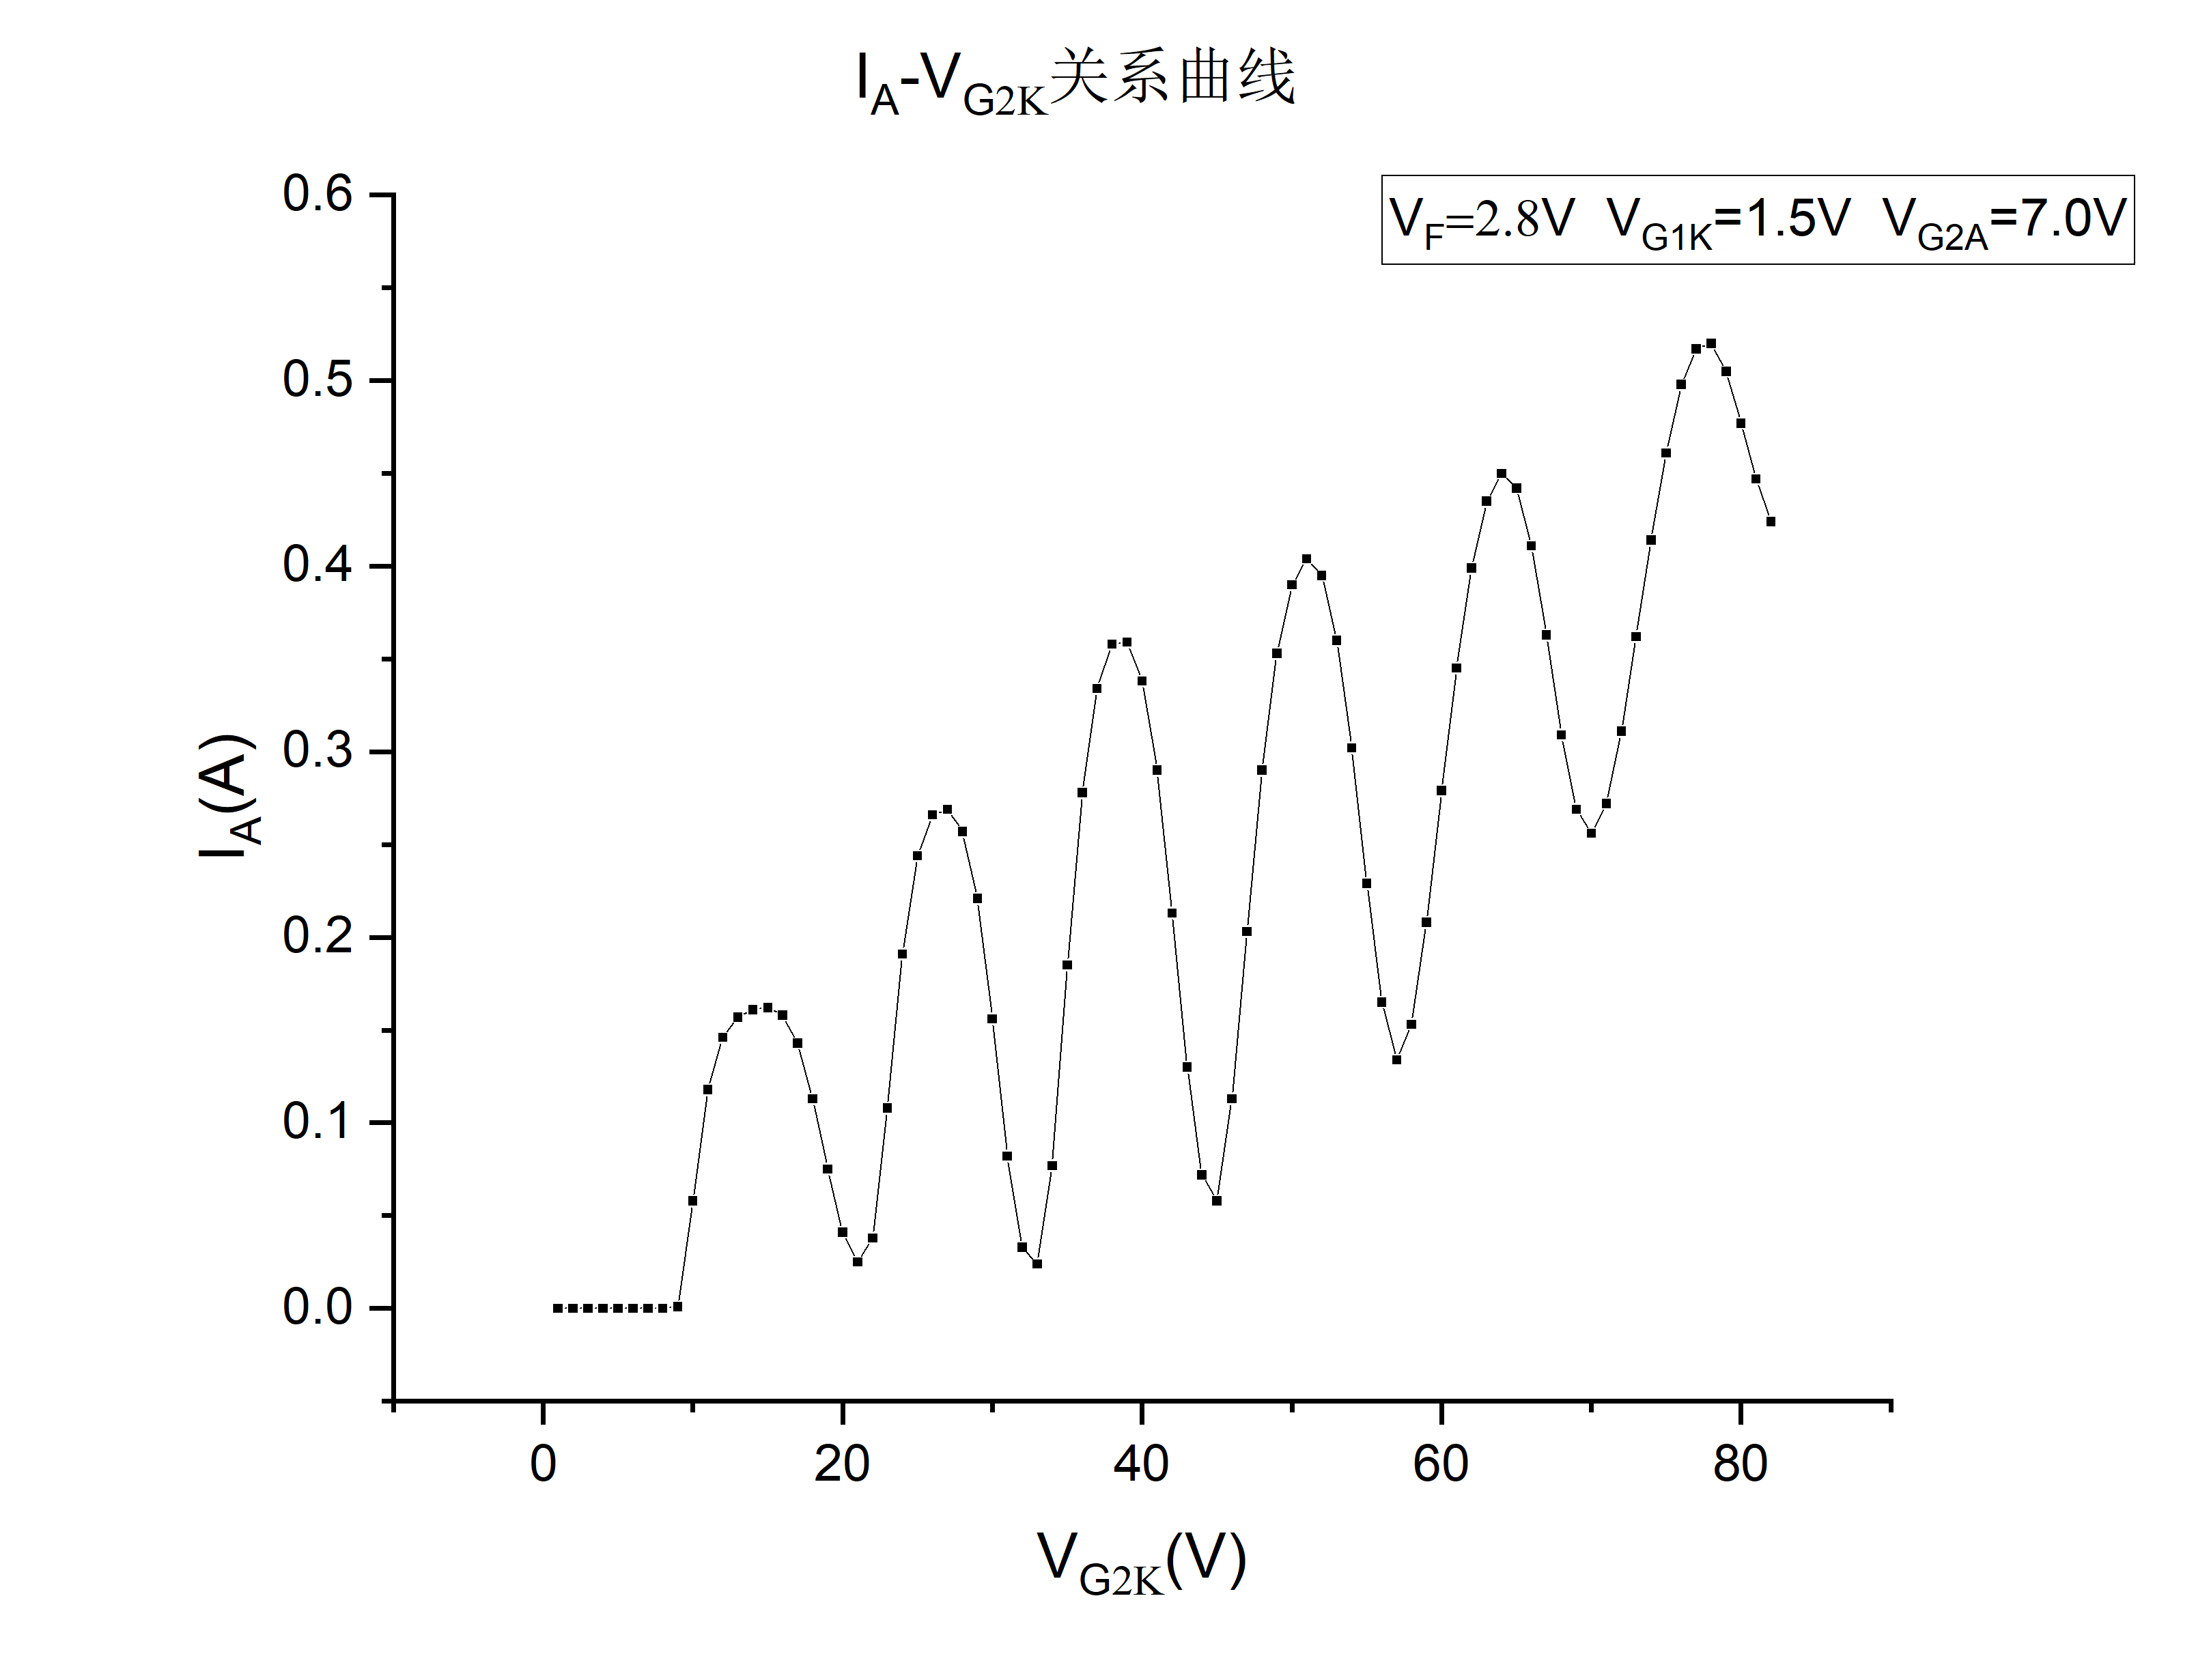
\includegraphics[width=0.5\textwidth]{img/3.1.png}%调节这里的图片宽度
		}%
		\subfloat[V$_{G1K}=2.0$时I$_{A}$-V$_{G2K}$关系曲线]{\label{fig:withgamma4}
		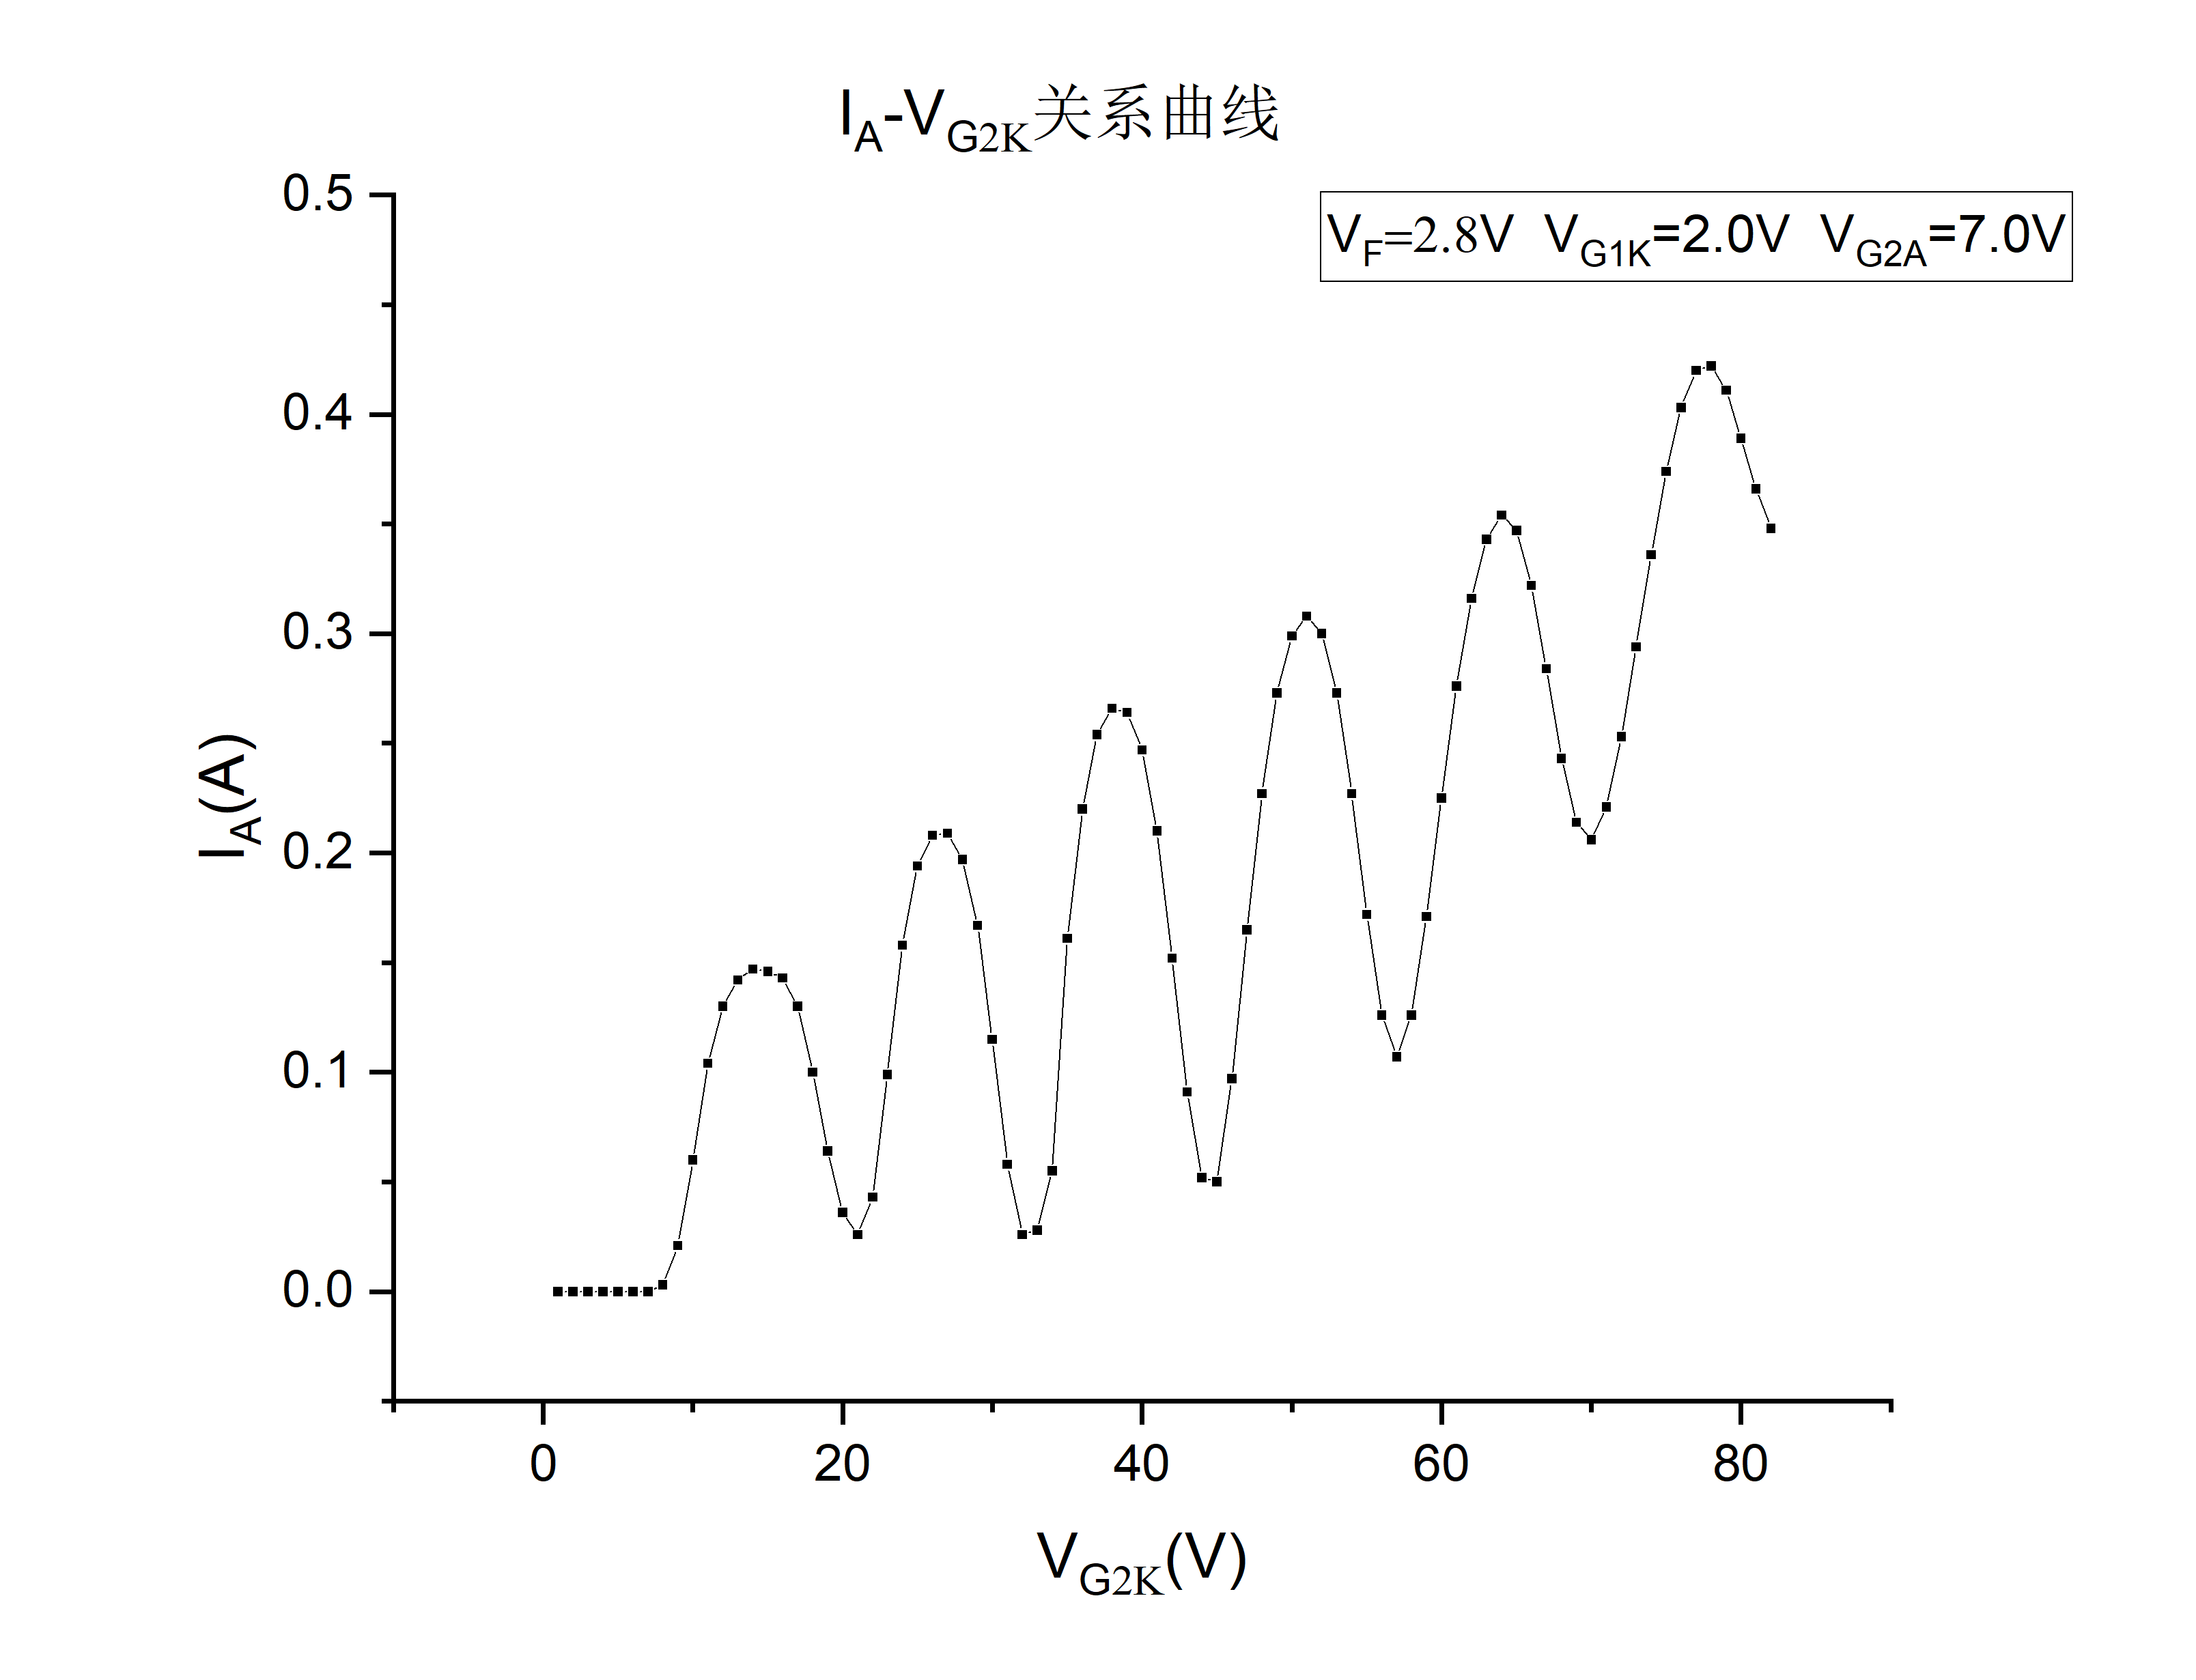
\includegraphics[width=0.5\textwidth]{img/3.2.png}%调节这里的图片宽度
		}%
		\caption{改变V$_{G1K}$时手动测量I$_{A}$-V$_{G2K}$关系曲线}
		\label{fig:tcvi}
	\end{figure}

	\begin{table}[htbp]
		\centering
		  \caption{第一激发电位}
		  \vspace{1em}
		\resizebox{\textwidth}{10mm}{%第一个大括号为宽度,第二个大括号为高度(60mm)可随机设置,调整到适合该表格的大小为止
		  \begin{tabular}{cccccccclcccccccc}
		  \toprule
		  极值点(a) & 1&2&3&4&5&6&均值&极值点(b) & 1&2&3&4&5&6&均值\\
		  \midrule
		  $V_{G2K} (V)$&14&27&39&51&64&78& & $V_{G2K}(V)$ &14&26&38&51&64&78& \\
		  $\varDelta V_{G2K}(V)$ & &13&12&12&13&14&12.8&$\varDelta V_{G2K}(V)$ & &12&12&13&13&14&12.8\\

		  \bottomrule
		  \end{tabular}}%注意这里还有一个半括号
		\label{tab:data}%
	  \end{table}

	由表一得:Ar元素的手动测量第一激发电位为12.8V。


	\subsubsection*{2.用示波器自动采集I$_{A}$-V$_{G2K}$关系曲线}
	
	对比不同工作电压下测得的 I$_{A}$-V$_{G2K}$ 曲线,作图并说明其异同,并说明各工作电压(V$_F$、V$_{G1K}$、V$_{G2A}$)的影响及原因。

	\begin{figure}[htbp]
		\centering
		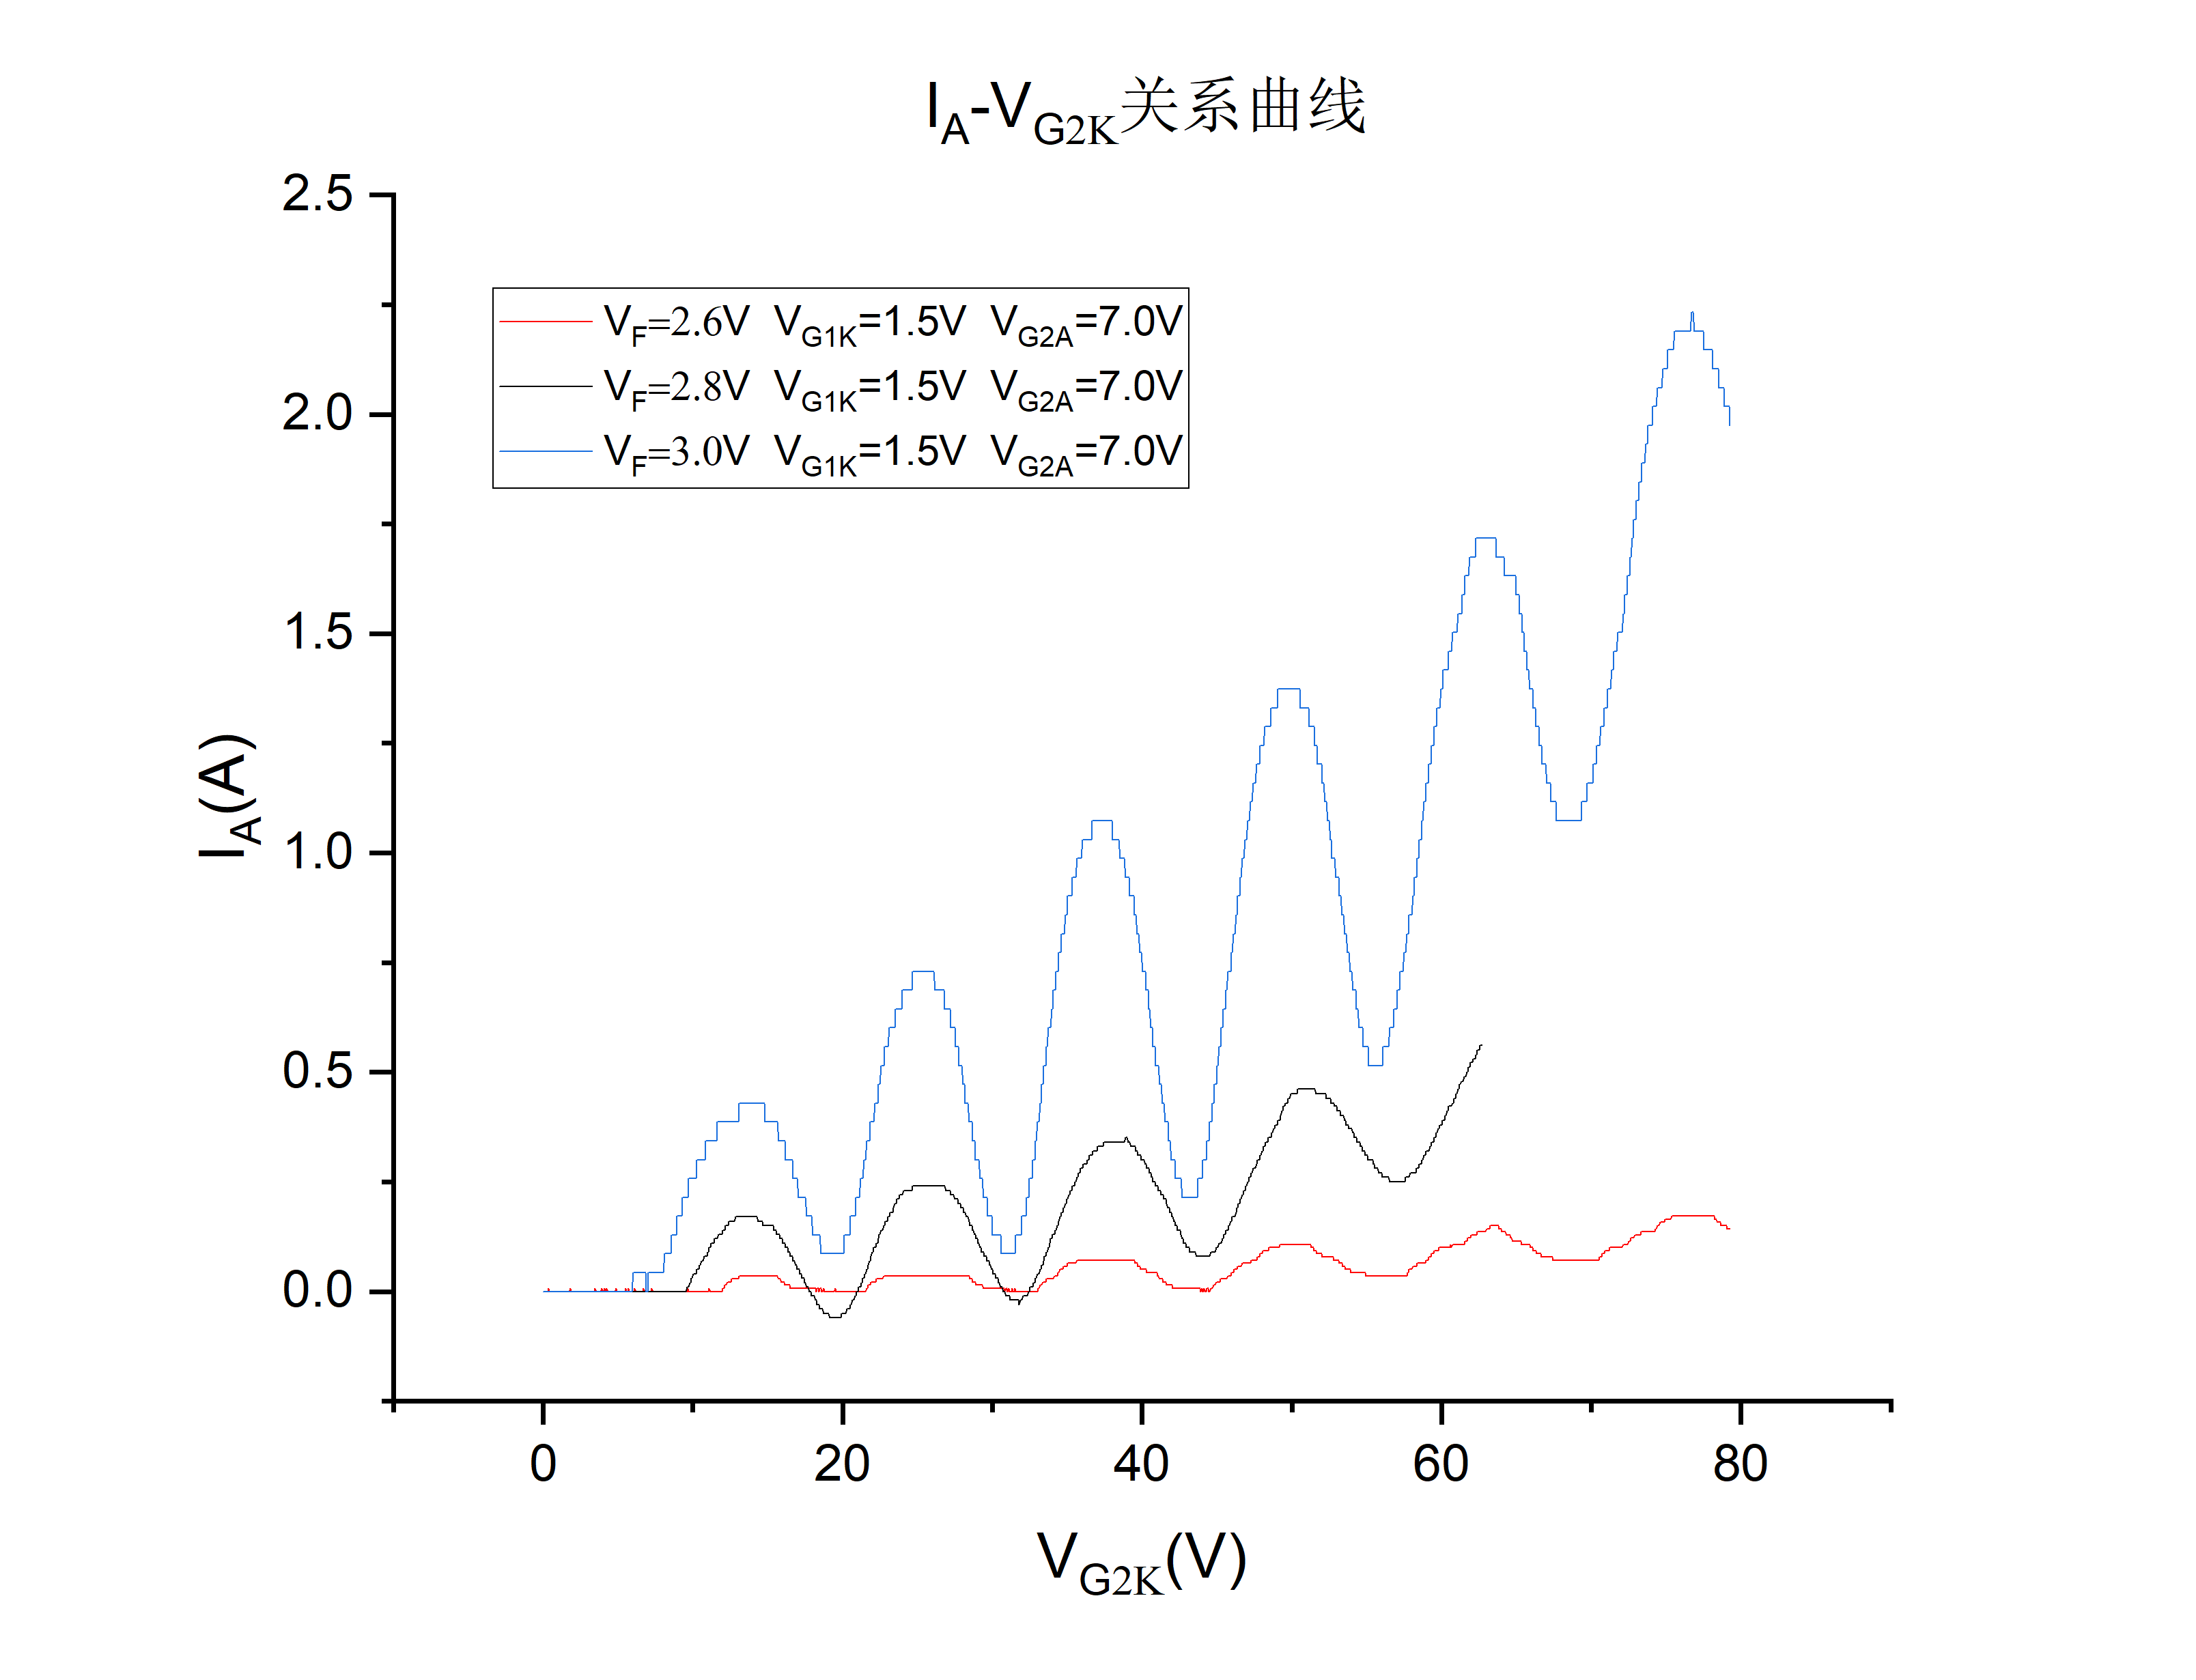
\includegraphics[width=0.8\textwidth]{img/4.1.png}
		\caption{改变V$_F$后I$_{A}$-V$_{G2K}$ 关系曲线}
	\end{figure}

	\paragraph*{(1)}
	保持V$_{G1K}$=1.5V,V$_{G2A}$=7.0V电压不变,改变V$_F$电压:

	由图4可知,灯丝电压V$_F$对I$_{A}$-V$_{G2K}$ 关系曲线有显著影响,总的来说V$_F$与阳极电流I$_A$基本成正比关系。
	当V$_F$较小时,I$_{A}$-V$_{G2K}$ 关系曲线呈平稳态势,无明显周期性变化;
	当V$_F$增加到足够大后,I$_{A}$-V$_{G2K}$ 关系曲线会交替出现呈周期性变化的极大值和极小值,不同灯丝电压对应的I$_{A}$-V$_{G2K}$ 关系曲线峰值出现的阳极电压V$_{G2K}$相同,各波峰与波谷之间的间距基本保持不变,证明了原子内部的能量状态的不连续性。
	并且V$_F$越大,相同的V$_{G2K}$所对应的I$_A$值越大,相邻波峰与波谷之间的差值也越大。

	\begin{figure}[htbp]
		\centering
		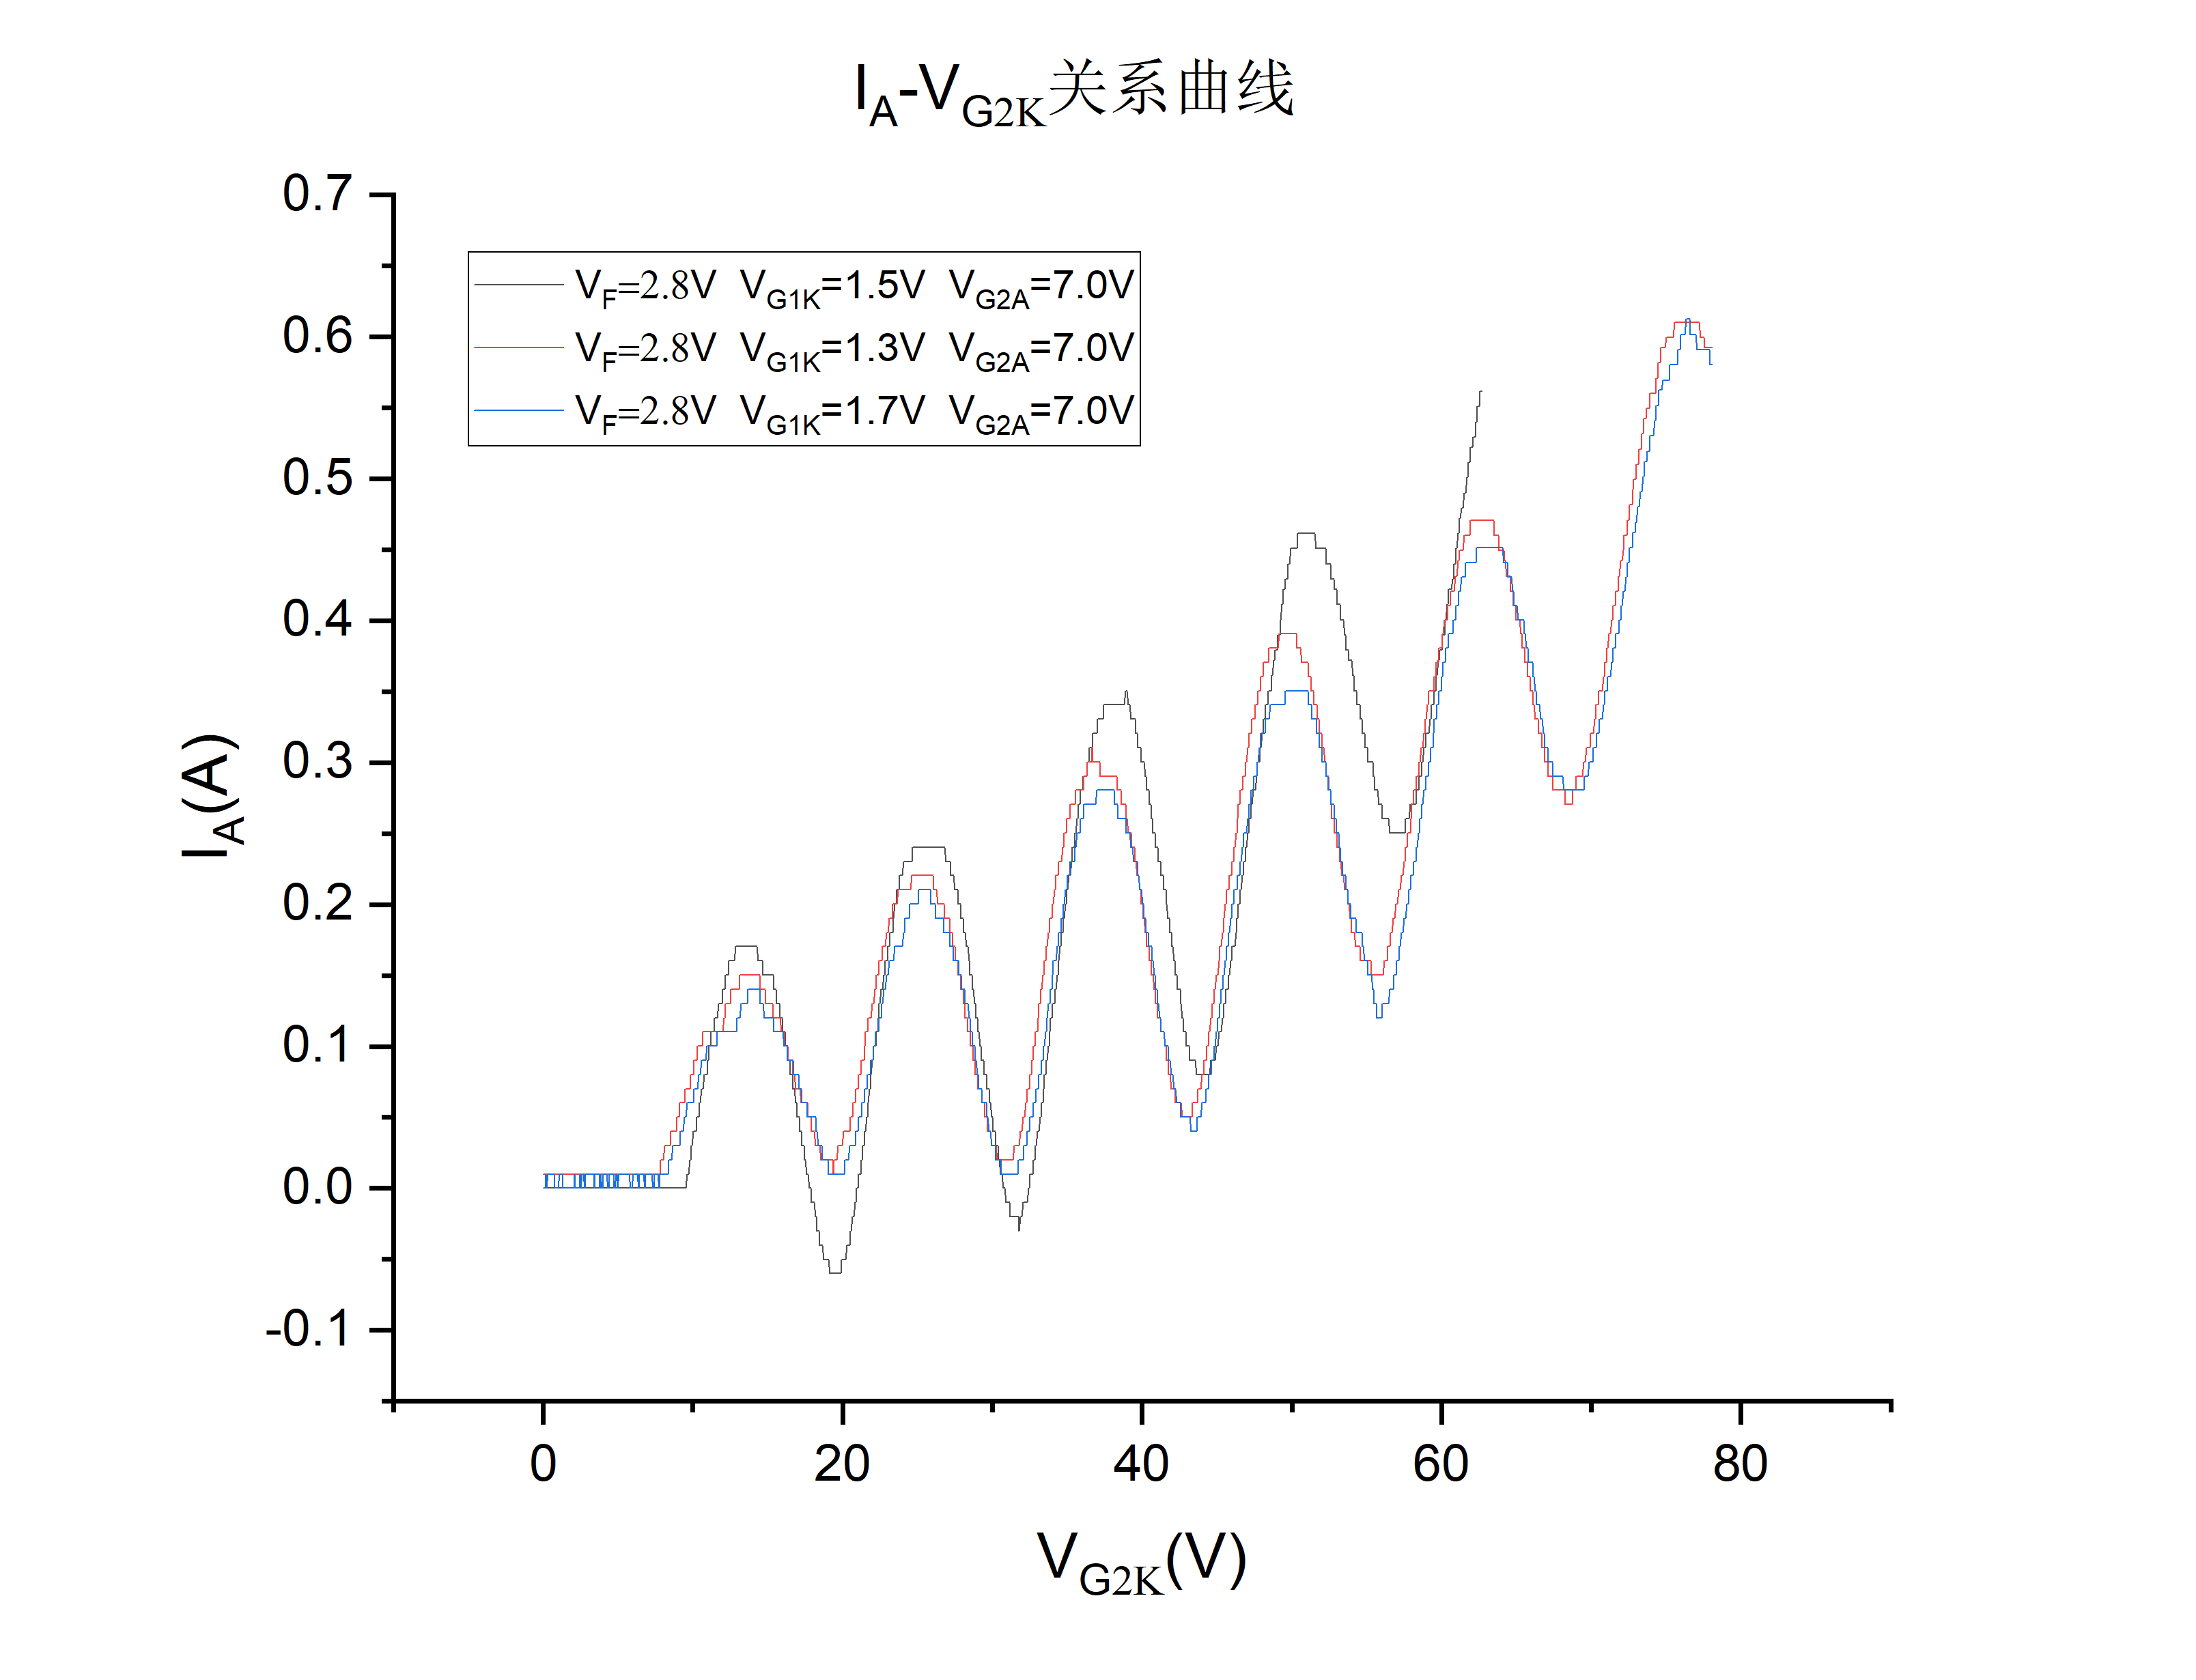
\includegraphics[width=0.8\textwidth]{img/4.2.png}
		\caption{改变V$_{G1K}$后I$_{A}$-V$_{G2K}$ 关系曲线}
	\end{figure}

	\paragraph*{(2)}
	保持V$_F$=2.8V,V$_{G2A}$=7.0V电压不变,改变V$_{G1K}$电压:

	由图5可知,不同的V$_{G1K}$值对实验曲线的影响并没有太大差异,尾部无明显上翘。

	\begin{figure}[htbp]
		\centering
		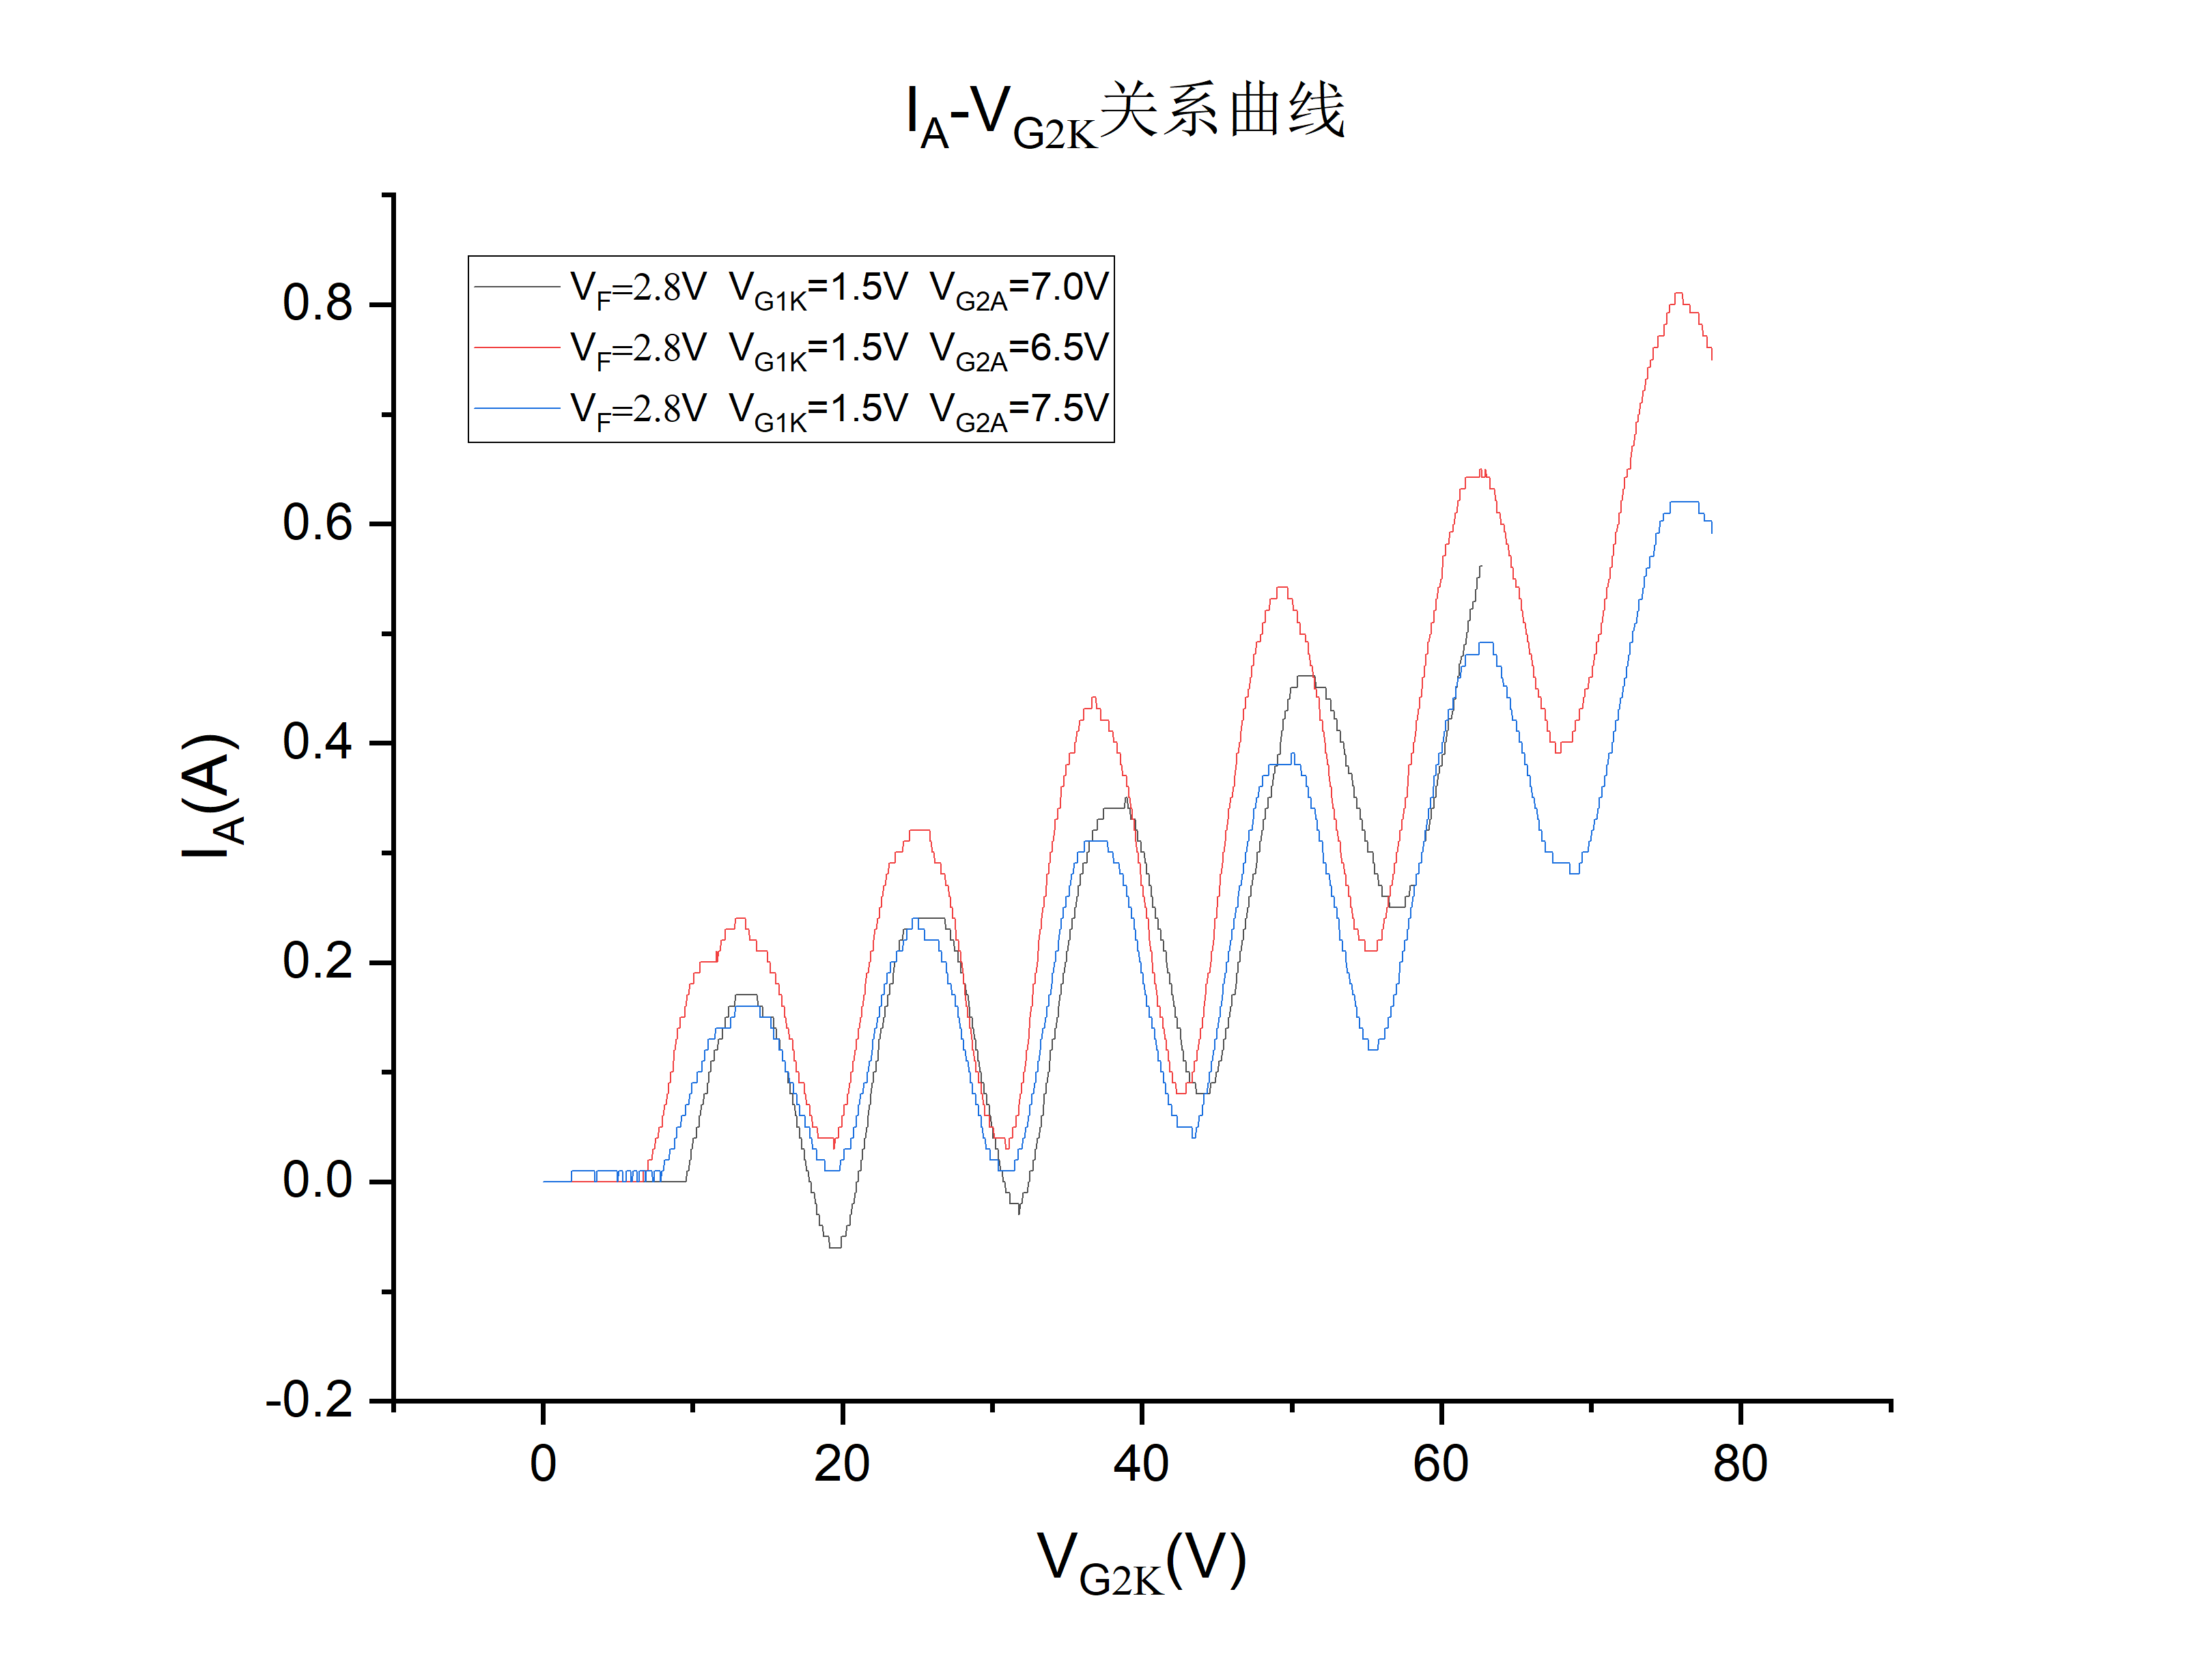
\includegraphics[width=0.8\textwidth]{img/4.3.png}
		\caption{改变V$_{G2A}$后I$_{A}$-V$_{G2K}$ 关系曲线}
	\end{figure}

	\paragraph*{(3)}
	保持V$_F$=2.8V,V$_{G1K}$=1.5V电压不变,改变V$_{G2A}$电压:

	由图6所示,不同V$_{G2A}$电压下I$_{A}$-V$_{G2K}$ 关系曲线的峰点位置有些差异,不过峰点间距大致相等。
	这是因为反向推迟电压越小,与氩原子碰撞后需要达到阳极A的能量越小,所以峰序对应的横坐标相对小;
	反之波峰对应的横坐标右移,即变大。
    反向推斥电压V$_{G2A}$越高,曲线的本底电流越小,峰值电压也略有下降。
    这是因为V$_{G2A}$可以将通过加速区而未达到阳极的电子推迟回栅极,起抑制本底电流的作用,减少电离。


\newpage

\subsection*{【思考题】}

	\subsubsection*{1.在数据处理的方法一中,直接取激发曲线中各峰(或谷)位间距的平均值作为第一激发电位值。这种方法是否合理?为什么? }
	答:这种方法有其合理性,但存在偏差。
	因为实验中存在本底电流的影响,本底电流是未与原子碰撞或与汞原子碰撞次数较少的电子形成的电流,所以各峰(谷)在激发曲线中的位置会收到本底电流的影响,而与实际位置略有偏差。由于本底电流随着加速电压的增大而增大,在加速电压比较大时各峰(谷)的位置偏离实际位置较远。
	因此,从需要从实验曲线中扣除本底电流的影响,再以差值曲线的各峰(谷)位间距作为第一激发电位值的方法比较合理。

	\subsubsection*{2.F-H管的I$_{A}$-V$_{G2K}$曲线中,相邻量波峰或波谷V$_{G2K}$之差表示什么?波峰为什么一定要有一定宽度?波谷点的 I$_A$为什么不等于零,且随V$_{G2K}$的增大而增大。}
	答:F-H管的I$_{A}$-V$_{G2K}$曲线中,相邻量波峰或波谷V$_{G2K}$之差表示原子的第一激发电位。
	电子在加速电压作用下能量是连续变化的,从而形成的阳极电流也是连续变化的,因此波峰会有一定的宽度。波谷点的I$_A$不等于零,是因为存在本底电流,随着V$_{G2K}$的增大,电子被加速得到的能量增大,速度增大,相同碰撞概率下有更多电子到达阳极。

	\subsubsection*{3.曲线中第一个波峰I$_{A}$-V$_{G2K}$是否就是第一激发电位?为什么?}
	答:不是。因为在第一个波峰处,电子还未能激发汞原子至第一激发电位。
	在本实验中,氩原子的第一激发电位对电子的影响表现在到达反射极的电子形成的电流的周期性变化上,只有相邻两波峰(谷)的V$_{G2K}$之差才是第一激发电位。

	\subsubsection*{4.何为F-H管的最佳工作方法,实验中需如何确定?}
	答:F-H管最佳工作点事选定一组合适的氩管工作电压,使I$_{A}$-V$_{G2K}$关系的峰位和谷位差异明显,本底电流得到较好的抑制,峰位拟合曲线尾部不出现明显上翘,拟合曲线呈纺锤状,此时这组工作电压称为最佳工作点。
	本实验在借助计算机和数据采集器快速采集大量数据的功能,定量研究F-H管个工作电压对I$_{A}$-V$_{G2K}$关系曲线的影响。
	在此定量研究的基础上,确定最佳工作点。

	\subsubsection*{5、如何定量描述F-H管各工作电压对I$_{A}$-V$_{G2K}$关系曲线的影响?}
	答:用控制变量的方法,每次只改变三个工作电压中的一个电压参数,另外两个保持不变。
\end{document}
